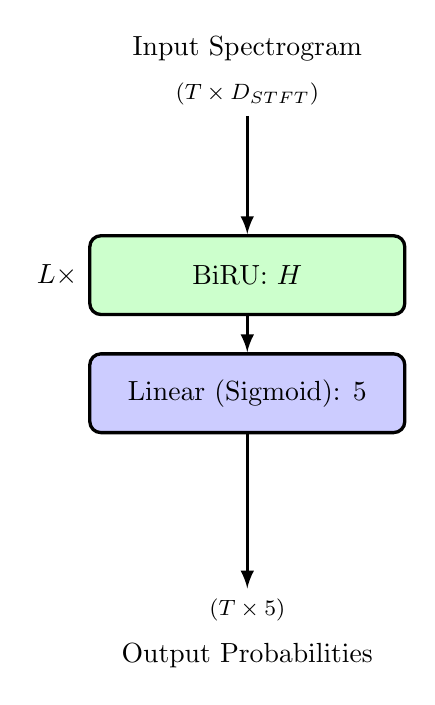
\begin{tikzpicture}[
    very thick,
    arrow/.style={
        -latex,
        very thick,
        rounded corners=0.2cm
    },
    ]

\node[anchor=south, label=above:{Input Spectrogram}] at (0, 0){\footnotesize{($T \times D_\text{STFT}$)}};

\draw[arrow] (0, 0) -- (0, -1.5) node[rectangle, 
rounded corners, 
draw, 
anchor=north, 
label=west:$L\times$,
fill=green!20,
minimum height=1cm,
minimum width=4cm
] (a) {BiRU: $H$};

\draw[arrow] (a) -- (0, -3) node[rectangle, 
rounded corners, 
draw, 
anchor=north, 
fill=blue!20,
minimum height=1cm,
minimum width=4cm
] (b) {Linear (Sigmoid): $5$};

\draw[arrow] (b) -- (0, -6);

\node[anchor=north, label=below:{Output Probabilities}] at (0, -6){\footnotesize{($T \times 5$)}};

\end{tikzpicture}